\section{Methods}\label{sec:methods}

\subsection{Data Pipeline}\label{sec:data-pipeline}

Training data was generated from DFT calculations on 51 closed-shell molecules drawn from the W4-11 thermochemistry benchmark set~\cite{karton2011w411}, spanning atomic species H, C, N, O, F, S, and Cl. All calculations used the LDA functional with MADNESS~\cite{harrison2016madness} multiresolution parameters $k=8$ (polynomial order) and $\epsilon = 10^{-6}$ (truncation threshold), matching production precision for the adaptive tree representation.

For each molecule, three MADNESS functions were generated in a three-step pipeline. First, \texttt{dump\_training\_functions} produced the superposition-of-atomic-densities initial guess $\rho_0(\mathbf{r})$ and the nuclear potential $V_\mathrm{nuc}(\mathbf{r})$ as MRA function trees serialized to HDF5. Second, \texttt{moldft} ran the SCF cycle to convergence. Third, \texttt{dump\_training\_functions -{}-archive} extracted the converged density $\rho(\mathbf{r})$ from the moldft checkpoint and wrote it as a third HDF5 tree. Each function is stored as a tree of $k^3 = 512$-element coefficient vectors (the \emph{s-coefficients}) at each node.

\paragraph{Sample construction.}
The dataset builder enumerates every node in the converged $\rho$ tree. Internal nodes (those with children) are labeled as positive samples requiring further refinement (\texttt{refine}=1); leaf nodes are positive samples that do not require refinement (\texttt{refine}=0). To provide negative examples, the builder generates the eight octree children below each leaf node by evaluating $\rho$'s s-coefficients at the child level via the two-scale relation (these children have vanishing wavelet coefficients by construction). The negative samples are labeled \texttt{refine}=0.

For each sample, the input features consist of (i) the $\rho_0$ and $V_\mathrm{nuc}$ s-coefficients at the box itself (each $k^3 = 512$ elements), (ii) the s-coefficients of $\rho_0$ and $V_\mathrm{nuc}$ at six face-adjacent halo boxes (each $6 \times 512$), and (iii) the integer tree level $n$. Halo s-coefficients for neighbors outside the simulation cell are zero-padded. The target is the converged $\rho$ s-coefficient vector at the same box. The complete HDF5 layout stores these arrays per molecule with gzip compression.

\paragraph{Train/val/test split.}
The 51 molecules were split by molecule: 45 for training, 3 for validation (ethanol, SO$_2$, HNNN), and 3 for testing (H$_2$O$_2$, C$_2$H$_2$, glyoxal). This molecule-level split ensures that the validation and test sets probe generalization to unseen geometries and electronic structures, not merely interpolation within a known tree. The 45 training molecules produced approximately 108,000 positive samples.

\subsection{Architecture (MRANet)}\label{sec:architecture}

MRANet is a FiLM-conditioned multilayer perceptron with a factored halo encoder (Figure~\ref{fig:architecture}).

\begin{figure}[htbp]
  \centering
  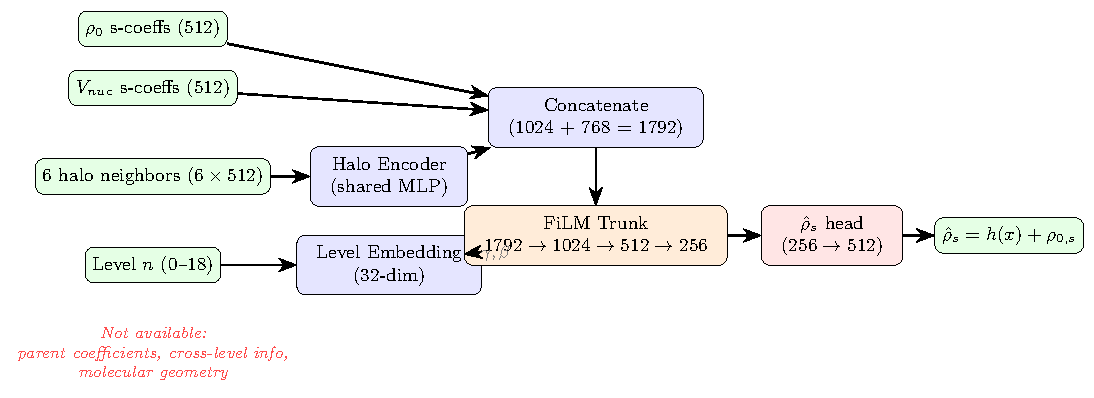
\includegraphics[width=\columnwidth]{figures/fig1_architecture.pdf}
  \caption{MRANet architecture. The model receives $\rho_0$ and $V_\mathrm{nuc}$ s-coefficients at the center box and six face-adjacent halo boxes, conditioned on the tree level via FiLM modulation. A residual connection adds the input $\rho_0$ coefficients to the network output.}
  \label{fig:architecture}
\end{figure}

\paragraph{Halo encoder.}
A shared MLP processes each of the six face-adjacent neighbor boxes identically. Each face's input is the concatenation of the neighbor's $\rho_0$ s-coefficients (512), $V_\mathrm{nuc}$ s-coefficients (512), and a learnable face embedding (8-dimensional, distinguishing $\pm x$, $\pm y$, $\pm z$ faces), giving an input dimension of 1032. The shared MLP maps this to a 128-dimensional output via one hidden layer of 256 units with ReLU activation. The six per-face outputs are concatenated to produce a 768-dimensional halo representation.

\paragraph{Center features.}
The s-coefficients of $\rho_0$ and $V_\mathrm{nuc}$ at the box itself are concatenated into a 1024-dimensional center feature vector.

\paragraph{FiLM conditioning.}
The tree level $n \in \{0, \ldots, 18\}$ indexes a 32-dimensional learned embedding table. At each trunk layer, a linear projection maps this embedding to a per-neuron scale $\gamma$ and shift $\beta$, applied after batch normalization following the FiLM mechanism~\cite{perez2018film}:
\begin{equation}
  \mathbf{h} = \gamma \odot \mathrm{BN}(W\mathbf{x} + \mathbf{b}) + \beta.
\end{equation}
This allows the network to adapt its behavior to the characteristic length scale and coefficient magnitude at each tree level without dedicating separate parameters per level.

\paragraph{Trunk.}
The halo representation and center features are concatenated into a 1792-dimensional input vector, which passes through three FiLM-conditioned layers with dimensions $1792 \to 1024 \to 512 \to 256$. Each layer applies a linear transformation, batch normalization, FiLM modulation, ReLU activation, and dropout ($p = 0.1$) in sequence.

\paragraph{Output head.}
A single linear layer maps the 256-dimensional trunk output to a 512-dimensional vector of predicted $\rho$ s-coefficients. The output uses a residual connection to the input $\rho_0$ s-coefficients:
\begin{equation}
  \hat{\rho}_s = f_\theta(\mathbf{x}) + \rho_{0,s},
\end{equation}
so the network learns the correction $\rho_s - \rho_{0,s}$ rather than the full density. This inductive bias reflects the physical expectation that the converged density is close to the atomic superposition guess. The single-task model contains approximately $3.04 \times 10^6$ parameters.

\subsection{Training and Inference}\label{sec:training}

\paragraph{Loss function.}
The single-task model was trained with a weighted mean squared error loss on the s-coefficient vector. To counteract the class imbalance (approximately 87\% negative samples in the dataset), positive (in-tree) samples received a weight of 10 relative to negative (below-leaf) samples. The loss also incorporated level-aware masking: tree levels with fewer than 200 training samples were excluded entirely (hard cutoff), and the remaining levels were weighted by $\sqrt{c_\ell / c_\mathrm{max}}$ where $c_\ell$ is the sample count at level $\ell$ and $c_\mathrm{max}$ is the maximum count across levels. This soft weighting prevented data-sparse levels from dominating the gradient.

\paragraph{Optimization.}
The model was trained with AdamW (learning rate $2 \times 10^{-4}$, weight decay $10^{-4}$) using a linear warmup over 5 epochs followed by cosine decay to a minimum learning rate of $10^{-6}$. Batch size was 4096 samples. Training used automatic mixed precision (AMP) with gradient scaling and ran for up to 120 epochs with early stopping (patience 20 epochs, monitored on validation loss).

\paragraph{Single-task inference.}
At inference time, \texttt{predict\_density\_simple()} copies the $\rho_0$ tree topology (preserving internal node structure and leaf set), replaces each leaf's s-coefficients with the model's prediction, then runs a compress-reconstruct pass to enforce two-scale consistency throughout the tree. The predicted tree is then scaled so that $\int \hat{\rho}(\mathbf{r})\,d\mathbf{r} = N_e$. Level clamping restricts model predictions to levels 10--14 (where training data is abundant), falling back to unmodified $\rho_0$ coefficients at all other levels.

\paragraph{SCF integration.}
The predicted density was injected into MADNESS's SCF solver as a replacement initial guess. The integration required three components: (i) a C++ modification to \texttt{SCF::initial\_guess()} in \texttt{SCF.cc} (approximately 20 lines) that detects a \texttt{rhoML} archive at startup, loads it via \texttt{ParallelInputArchive}, and rescales to the correct electron count, falling back to the standard $\rho_0$ if the archive is absent; (ii) an \texttt{h5\_to\_archive} converter that reads the HDF5 function tree produced by Python-side inference and writes a MADNESS binary archive compatible with the C++ reader; and (iii) a driver script that runs ML inference, converts the output, and launches \texttt{moldft} with the ML-derived initial guess alongside a baseline run for comparison.
